\documentclass[10pt]{report}

%% Language and font encodings
\usepackage[english]{babel}
\usepackage[utf8x]{inputenc}
\usepackage[T1]{fontenc}
\usepackage{url}
\usepackage{setspace}
\renewcommand{\baselinestretch}{1.2}

%% Sets page size and margins
\usepackage[a4paper, top=2cm, bottom=2cm, left=2cm, right=2cm, marginparwidth=1.75cm]{geometry}

%% Useful packages
\usepackage{graphicx}
\usepackage{makeidx}    % allowsindexgeneration
\usepackage{float}
\usepackage{acronym}
\usepackage{hyperref}

\pagenumbering{arabic}

\begin{document}
\thispagestyle{empty}

\begin{figure}[h]
    
\includegraphics[width=0.45\textwidth]{assets/logo.png}
\end{figure}

\begin{center}


    \begin{Huge}
        \textbf{SCAR\@: Smart Contract Academic \\ \vspace{.25cm}
            Registry}
    \end{Huge}

    \vspace{.75cm}

    \begin{LARGE}
        \textbf{A Blockchain approach for Academic Registry}
    \end{LARGE}

    \vspace{1cm}

    \vspace{.75cm}
    \begin{large}
        \begin{tabular}{ c c c }
            Diogo Rodrigues               & Gonçalo Frutuoso              \\
            \texttt{49513@alunos.isel.pt} & \texttt{49495@alunos.isel.pt} \\
        \end{tabular}

        \vspace{5.75cm} Supervisors \vspace{0.25cm}

        \begin{tabular}{ c c }
            Cátia Vaz, ISEL              & Alexandre Francisco, IST \\
            \texttt{cvaz@cc.isel.ipl.pt} & \texttt{aplf@tecnico.pt}
        \end{tabular}

        \vspace{1.25cm}

        \begin{Large}
            Final Report written for Project and Seminary \\ \vspace{.25cm}
            Licenciatura em Engenharia Informática e de Computadores
        \end{Large}
    \end{large}

    \vspace{1.75cm} \today \vspace{.75cm}

\end{center}

% Empty page before the abstract
\newpage
\thispagestyle{empty}
\mbox{}

%%%%% Abstract %%%%%
%
% Abstract
% 
\chapter*{Abstract}\label{chap:abstract}

A major difficulty in the digital age of today is verifying the legitimacy of academic credentials. Significant issues facing the education sector include the pervasive problem of phony credentials and the absence of a reliable, global system for confirming academic accomplishments. The verification procedure is often complicated by traditional systems, which are dependent on specific educational institutions. This might raise questions regarding the authenticity of academic records. Professionals must also refresh and validate their abilities on a regular basis, but there aren't enough trustworthy venues to display these competencies.

In this research, an innovative solution utilizing blockchain technology to address these difficulties is presented: the DiGo Certify App. This App ensures fraud-proof procedures by utilizing smart contracts to automate and secure academic credential validation and issuing.

Designed to comply with the General Data Protection Regulation (GDPR), this system empowers individuals with control over their personal data while maintaining the integrity and transparency of academic records.

The DiGo Certify App integrates smoothly with existing institutional systems, avoiding the need for significant upgrades. It is versatile enough to certify various types of academic information, covering both formal qualifications and informal learning. This work examines the advantages and implications of this model, emphasizing the crucial role of privacy and data protection in blockchain-based educational solutions.

\paragraph{Keywords:} Academic Credential Verification, Blockchain Technology, Smart Contracts, DiGo Certify App, Fraud Prevention, GDPR Compliance, Educational Records, Data Privacy, Academic Certification, Digital Education Solutions

% Empty page before the resumo
\newpage
\thispagestyle{empty}
\mbox{}

%%%%% Resumo %%%%%
%
% Resumo
%
\chapter*{Resumo}\label{chap:resumo}

Aqui fica o resumo.

% Empty page before the acknowledgements
\newpage
\thispagestyle{empty}
\mbox{}

%%%%% Acknowledgements %%%%%
% %
% Acknowledgments
%
\chapter*{Acknowledgments}\label{chap:acknowledgments}

Here goes the acknowledgments.

%%%%% Index %%%%%
\renewcommand{\contentsname}{Index}
\pagenumbering{arabic}
\tableofcontents

%%%%% List of figures %%%%%
\listoffigures
\addcontentsline{toc}{chapter}{List of Figures}

%%%%% List of tables %%%%%
\listoftables
\addcontentsline{toc}{chapter}{List of Tables}

%%%%% List of acronyms %%%%%
\chapter*{List of Acronyms}
\addcontentsline{toc}{chapter}{List of Acronyms}

\begin{acronym}[TDMA]
    \acro{BTC}{Bitcoin}
    \acro{dApps}{Decentralized Applications}
    \acro{RPOW}{Reusable Proof of Work}
    \acro{PoW}{Proof-of-Work}
    \acro{PoS}{Proof-of-Stake}
    \acro{WEB3}{Web 3.0}
    \acro{EVM}{Ethereum Virtual Machine}
    \acro{CLI}{Command Line Interface}
    \acro{KMP}{Kotlin Multiplatform}
    \acro{Admin}{Administrator}
    \acro{UI}{User Interface}
    \acro{SDK}{Software Development Kit}
    \acro{HTTPS}{ Hypertext Transfer Protocol Secure}
    \acro{ABI}{Application Binary Interface}
    \acro{ERC}{Ethereum Request for Comments}
    \acro{SHA}{Secure Hash Algorithm}
    \acro{JSON}{JavaScript Object Notation}
    \acro{RSA}{Rivest-Shamir-Adleman}
    \acro{OnchainID}{On-Chain Identity}
    \acro{IPFS}{InterPlanetary File System}
    \acro{T-REX}{Tokenized Real Estate Exchange}
\end{acronym}


%%%%% CHAPTERS (with an empty page before each one) %%%%%
\newpage
\thispagestyle{empty}
\mbox{}
%
% Chapter 1
%
\chapter{Introduction}\label{chap:introduction}

With the advent of the digital era, the management of academic records presents substantial challenges. The prevalence of forged certificates and the absence of a universally trusted system for issuing and verifying academic credentials contribute to significant issues within the education sector. Traditionally, academic records are managed by individual institutions through their proprietary systems, making verification by external stakeholders cumbersome. This lack of transparency and accessibility complicates the process of confirming the authenticity of academic accomplishments, leading to potential mistrust and inefficiencies.

The inability to effectively verify academic credentials has facilitated the rise of degree mills~\cite{saleh2020blockchain}, which produce counterfeit certifications. These fraudulent activities undermine the credibility of genuine academic institutions and compromise the value of legitimate degrees~\cite{muzammil2010corrupt}. Furthermore, the current systems are susceptible to unauthorized alterations and inaccuracies, further eroding trust in academic records.

To address these challenges, it is essential to explore and compare the different types of academic certificate storage and verification systems. The first type is the traditional database system~\cite{OLSON200971}, presented in Section~\ref{sec:centralized-systems}, where records are stored in centralized databases managed by individual institutions.
While this method provides control to institutions, it often has a gap in the necessary security and accessibility features to prevent fraud and ensure efficient verification.

The second type of solution is presented in Section~\ref{sec:distributed-systems} and involves distributed systems, which use multiple servers to manage records across various nodes.
This approach enhances security and reduces the risk of data loss but still relies on trusted intermediaries, which can introduce vulnerabilities and inefficiencies.

The third and most innovative solution is the fully distributed system, described in Section~\ref{sec:blockchain} using \textit{blockchain technology}. Blockchain~\cite{saleh2020blockchain} offers a decentralized and tamper-proof method for recording and verifying academic credentials.
By leveraging smart contracts, academic records can be securely issued, stored, and verified on a blockchain. This approach ensures transparency, reduces the risk of fraud, and simplifies the verification process for stakeholders.

The SCAR project represents an innovative application of blockchain technology in the education sector. This system aims to streamline the issuance and verification of academic certificates, ensuring that all records are securely stored and easily accessible for verification. The use of smart contracts in the DiGo Certify App automates the process of certificate issuance and validation, making it efficient and tamper-proof.

Moreover, compliance with data protection regulations, such as the General Data Protection Regulation (GDPR), is a critical aspect of this solution. The DiGo Certify App is designed to adhere to GDPR principles, ensuring that personal data is protected while maintaining the integrity and transparency of academic records on the blockchain.

Through the SCAR project and the DiGo Certify App, we aim to demonstrate how blockchain technology can revolutionize academic credential management, providing a secure and transparent system for the future.

\newpage
\thispagestyle{empty}
\mbox{}
%
% Chapter 2
%
\chapter{Background}\label{chap:background}
\paragraph{}

Nowadays, the authenticity and accessibility of academic certificates play a crucial role in ensuring trust and credibility in various
domains, ranging from education to employment and beyond.
The current and traditional \textit{paper-based} system of issuing and verifying academic certificates is not only time consuming but also prone to a lot of fraud and manipulation.
The widespread issue of counterfeit certificates\cite{certCounterfeitAdv, certCounterfeitRid}, coupled with inefficient verification processes and the risk of loss or damage, highlight the need for a more reliable and secure academic certificate registry system.

The current system of academic certificate registry faces numerous challenges. Firstly, the reliance on paper-based is problematic. Paper-based certificates are easily forged and tampered with. This undermines the credibility and integrity of academic qualifications. Secondly, the manual verification process is
time-consuming and prone to errors, leading to delays in credential validation, possible fraudulent activities and also potential loss of revenue for institutions due to
errors in the manual release. Thirdly, since the issue of certificates from educational institutions are mostly centralized, this intensify the difficulty
of maintaining a unified and updated registry, avoiding efficient verification mechanisms.

\section{Overview}\label{sec:overview}
\paragraph{}

There are several approaches to address the challenges of the traditional academic certificate registry system. One such solution is the implementation of centralized databases managed by government or regulatory authorities,
where educational institutions are required to submit digital copies of certificates for verification purposes~\cite{LinWays}.
Other solution is the adoption of distributed systems where the data is stored across multiple nodes in a network, but not all nodes have the same equal authority and the data is not fully decentralized. Which means that there's an entity that has control over the network~\cite{sharples2016blockchain}.
This solution is not centralized neither fully distributed but have a mix of both approaches that makes the system more secure and reliable than only a centralized one.
The third solution that we will approach is a fully distributed one that offers a decentralized, secure and tamper-proof ledger where certificates can be stored and verified where
there is no single entity that has control over the network. This solution is based on the \textit{blockchain technology}~\cite{app14020706, saleh2020blockchain}.

\section{Centralized Systems}\label{subsec:centralized-systems}
\paragraph{}

Several attempts have been made to address the challenges of the traditional academic certificate registry system.
How we can see in the Figure~\ref{fig:centralized-system}, one such solution is the implementation of \textit{centralized databases}~\cite{OLSON200971} managed by government or regulatory authorities, where educational institutions are required to
submit digital copies of certificates for verification purposes. Although this approach aims to centralize certificate records and simplify the verification process, it still faces challenges
such as the risk and concerns of data privacy and security, interoperability issues between different databases and the need of a trusted third party to manage the database.
This centralized systems often only store grades and not the actual certificates which undermines the credibility and integrity of academic qualifications.
Moreover, the reliance on a central authority to manage the registry increases the risk of fraud and manipulation, as the data can be altered or deleted by a single entity.

\begin{figure}[H]\label{fig:centralized-system}
    \begin{center}
        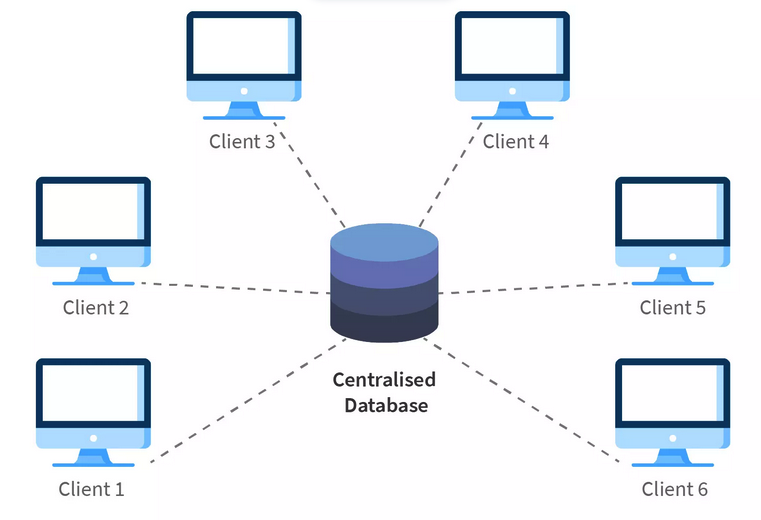
\includegraphics[width=0.8\textwidth]{assets/centralized-database.png}
        \caption{Centralized System~\cite{centralizedDB}.}
    \end{center}
\end{figure}

\section{Distributed Systems}\label{subsec:distributed-systems}
\paragraph{}

Another solution to address the challenges of the traditional academic certificate registry system could be the adoption of distributed systems where the data is stores in multiple nodes in a network.
Has we see in the Figure~\ref{fig:distributed-system}, different that what we've seen in the previous section, the data is replicated across multiple nodes of the system, ensuring that the data is available even if some nodes fail. However, not all nodes have the same equal authority which means that
it is not fully decentralized.

\vspace{.25cm}
\begin{figure}[h]\label{fig:distributed-system}
    \begin{center}
        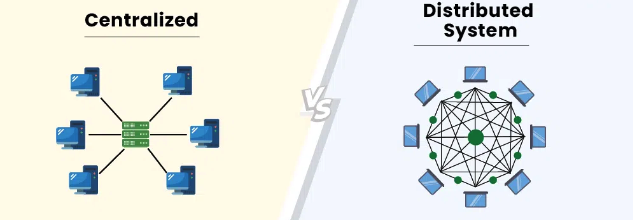
\includegraphics[width=0.8\textwidth]{assets/centralized-vs-distributed.png}
        \caption{Centralized vs Distributed Systems~\cite{centralizedVsDistributed}.}
    \end{center}
\end{figure}

In the context of education, distributed systems can significantly enhance the reliability and security of academic certificate validation.
Educational institutions, accrediting bodies, and employers can benefit from a system where academic records are distributed across a network of trusted nodes,
rather than being stored in a single central repository.
The key benefits of this approach in the education sector include improved security, enhanced reliability and scalability.

\section{Blockchain}\label{sec:blockchain}
\paragraph{}

Recently, another solution that have being proposed is the adoption of blockchain technology for academic certificate registry. As we can see in Figure \ref{fig:blockchain-vs-database}, also being a distributed system, this technology goes beyond by offering a fully decentralized solution.
Blockchain offers a decentralized, secure and \textit{tamper-proof ledger} where certificates can be stored and verified.
Tamper-proof ledger is a system designed to maintain records where once information is added, it cannot be altered or deleted. This is achieved through a combination of cryptographic techniques and a distributed network of computers (nodes) that each hold a copy of the ledger.
Every transaction or entry is verified by these nodes, and any attempt to change past records would require altering the data on a majority of these nodes simultaneously, which is virtually impossible. This ensures the integrity and authenticity of the stored certificates, making them highly resistant to fraud and manipulation.

\begin{figure}[H]\label{fig:blockchain-vs-database}
    \centering
    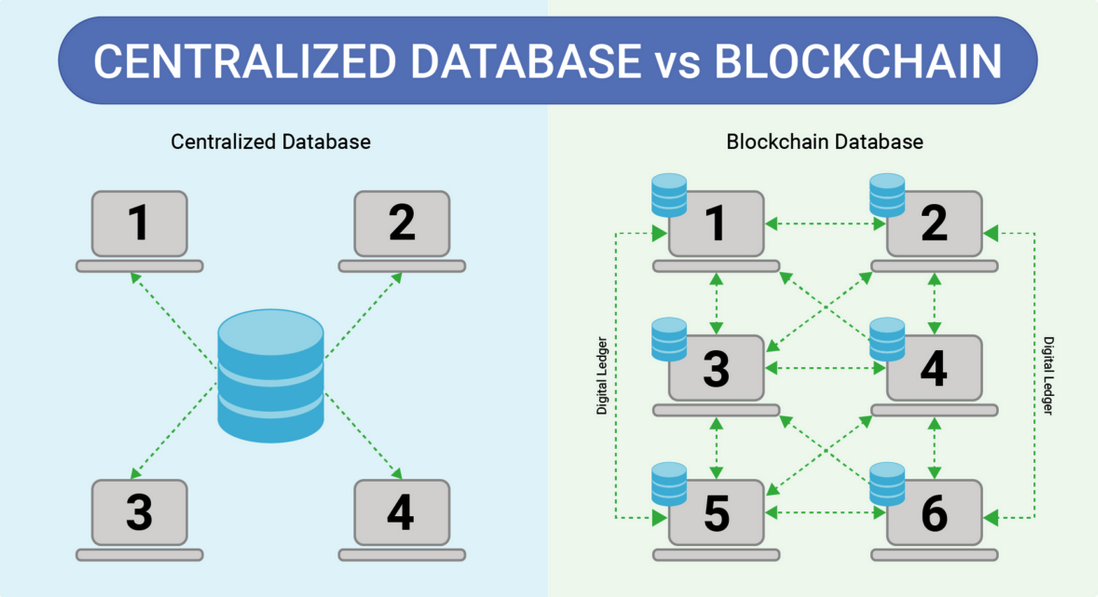
\includegraphics[width=0.8\textwidth]{assets/blockchain-vs-database.png}
    \caption{Centralized vs Blockchain Systems~\cite{blockchainDB}.}
\end{figure}

The use of blockchain technology ensures that certificates are immutable, transparent and accessible to all stakeholders~\cite{alammary2019blockchain}. Moreover, this technology enables the instant verification through cryptographic methods,
eliminating the need for a central authority to manage the registry, thereby reducing the risk of fraud and manipulation.

In contrast to the traditional centralized data-based system, in our opinion, blockchain emerges with a huge influence capable of revolutionizing academic certificate registry systems.
The decision to use blockchain technology as the foundation of our solution on the fact that blockchain technology is a key enabler of the \textit{Web3} vision~\cite{buldas2022towards},
which aims to create decentralized and fully distributed applications (\textit{dApps}) that are secure, transparent and trust less where users have full control over their data and digital assets without having a \textbf{single point of failure}.
For the implementation of a blockchain-based solution for our problem it is crucial to understand the foundational concepts that make this technology both revolutionary and reliable.
Central to blockchain's efficacy is the principle of \textit{distributed consensus}~\cite{xiao2020survey}, which ensures the integrity, security and transparency of the ledger like mentioned before.

% Should we add a subsection here where walk deeper into the blockchain technology and its concepts?

Blockchain technology started to gain popularity in 2008 initially described by Satoshi Nakamoto in a white paper entitled `Bitcoin: A Peer-to-Peer Electronic Cash System'~\cite{nakamoto2008bitcoin}.
Although the term blockchain gained popularity in that year, with the introduction of Bitcoin cryptocurrency by Nakamoto, its underlying concepts have been used since the 1980s.
Later in 2004, Harold Thomas Finney II introduced the Reusable Proof of Work (\textit{RPOW}) system~\cite{RPOW}. The RPOW system was a digital
currency system that used a \textit{proof-of-work} that limit the amount of work done by the server and to limit the amount of work done by the client.
The RPOW system was the first system to use a blockchain-like structure to store and verify transactions. Later, in 2009 the first bitcoin transaction was made by Nakamoto
to his friend Hal Finney~\cite{peterson2014hal} where was transferred 10 BTC (bitcoin). This marked the beginning of the blockchain technology era.
In 2013, Vitalik Buterin proposed the concept of \textit{smart contracts} in his white paper `Ethereum: The Ultimate Smart Contract and Decentralized Application Platform'~\cite{buterin2013ethereum}. Upon this publication,
\textit{Ethereum} has launched his own blockchain in 2015.~\cite{reiff2020bitcoin}.

Blockchain can be defined as a time-ordered set of blocks or nodes where each block is cryptographically linked to the previous one forming a chain. All blocks are stored in a decentralized and distributed ledger and become
trustworthy digital records what are unmodifiable in practice but very easy to verify. Like mentioned before, there is no centralized or hierarchical structure in the blockchain network and the information is shared by a network of \textit{peers}.

\begin{figure}[h]\label{fig:blockchain}
    \begin{center}
        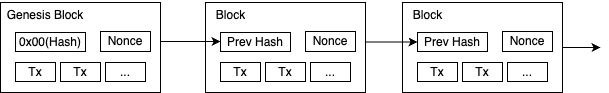
\includegraphics[width=0.8\textwidth]{assets/blockchain.png}
        \caption{Blockchain structure adapted from~\cite{nakamoto2008bitcoin}}
    \end{center}
\end{figure}

As it can be observed in Figure~\ref{fig:blockchain}, each block contains a reliable register of one or more actually executed transactions that are created and exchanged by the network participants (peers) which eventually must modify
its state. To add new information to the chain, a \textbf{consensus} (\ref{subsec:distributed-consensus-mechanisms}) about its truthfulness must be reached among the peers in the network.

The content of each transaction that is stored in a single block depends on the specific type of blockchain and its purpose. In our case and very succinctly, the transaction has an `item' that contains information about the academic certificate; we will discuss this in more detail in the next chapters. Other example used nowadays is the Bitcoin, where the main information registered in transactions are exchanges of bitcoins between accounts.

Other important aspect of a chain node and the major reason for its security is the \textbf{hash} function.
This function is used like a digital fingerprint to verify whether or not the data contained in the block has been tampered with. It is created when a new block is added or updated onto the chain.
In the blockchain, each block's hash includes the hash of the previous block, linking them together in a chain. If someone tries to change any information in a block, even just a tiny bit, the hash of that block will change completely. This change would break the link to the next block, making it obvious that the information has been tampered with.
This is the reason why the blockchain is considered tamper-proof and secure.

Some blockchains support the use of \textit{Smart Contracts}~\cite{kaur2023introduction} which are self-executing contracts with the terms of the agreement directly written into code.
These Smart Contracts are a critical component of several applications and platforms using a distributed ledger technology that we will be using in our solution and for better understanding we will explain with
more detail in the next sections.

There are three main types of blockchain~\cite{paul2021blockchain}:

\begin{itemize}
    \item {Public}: is called public if each participants can read and use it to carry out transactions but also
          if everyone can participate in the process of creating the \textbf{consensus} which can be \textit{Proof-of-Work} or \textit{Proof-of-Stake}.
          In this type of blockchain there is no central authority nor a trusted third party to control the network.
          Examples of this type of blockchain are \textbf{Bitcoin}~\cite{nakamoto2008bitcoin} and \textbf{Ethereum}~\cite{tual2015ethereum}. The main advantages of this type of blockchain are:
          \begin{itemize}
              \item High security and privacy,
              \item Open and Flexible Environment,
              \item No regulations,
              \item Full Transparency and Systems,
              \item Distributed, etc.
          \end{itemize}

    \item {Private}: these are restricted and not open, such kind of blockchain also has features of access. This type of blockchains works mostly on closed systems and networks and are usually
          useful in organizations and companies which only selected members can join and access the data. Private blockchains have running only authorized nodes and that means that no one from the outside
          of the private network is able to access the information and data exchanged between two nodes. In this type there is no mining, no proof of work, and no remuneration~\cite{guegan:halshs-01524440}.
          Examples of this type of blockchain are \textbf{Hyperledger Fabric}~\cite{hyperLedger} and \textbf{R3 Corda}~\cite{r3Corda}.
          The main advantages of this type of blockchain are:
          \begin{itemize}
              \item Full of privacy,
              \item High Efficiency,
              \item Faster Transaction,
              \item Better Scalability,
          \end{itemize}
    \item {Consortium~\cite{KASI20221}}: a combination of both public and private blockchains. As in a private blockchain, participants may join the network only by invitation and must be approved by the network owner, however,
          there is not a single organization that has control over the network. Instead, the control is distributed among a group of participants.
          \begin{itemize}
              \item High Security,
              \item High Scalability,
              \item High Efficiency,
              \item High Privacy,
              \item High Flexibility,
          \end{itemize}

\end{itemize}

\subsection*{Distributed Consensus Mechanisms}\label{subsec:distributed-consensus-mechanisms}
\paragraph{}

As mentioned in the beginning of the section~\ref{sec:blockchain}, the blockchain technology is based on the concept of distributed consensus, which is a procedure used to achieve an
agreement among all the peers of the blockchain network about the present state of the ledger. Through this mechanism, consensus algorithms ensure that all nodes in the network agree on the validity of the transactions and the order in which they are added to the blockchain.
To do a parallelism with the real world, the consensus mechanism is the way that humans agree on the rules of a game, for example, in Monopoly where there are a lot of different ways to win, buying all the properties or end up with a lot of money in the bank
and bankrupt all the other players but no matter what the rules are, everyone has agreed that it is a fair way to end the game~\cite{whatIsConsensus}.
Consensus mechanisms are essential to the security and integrity of the blockchain network, as they prevent malicious actors from altering the ledger and ensure that all transactions are valid and consistent across all nodes.
It prevent the \textit{double-spending} problem, where a user spends the same digital currency more than once, which is a common issue in digital currency systems.

\begin{itemize}
    \item \textbf{Proof-of-Work (PoW)}: is the first consensus algorithm used in blockchain technology, introduced by Nakamoto in the Bitcoin white paper~\cite{nakamoto2008bitcoin}.
          In this mechanism, miners compete to solve complex mathematical puzzles to validate transactions and add new blocks to the blockchain. The first miner to solve the puzzle is rewarded with a certain amount of cryptocurrency.
          PoW is known for its high energy consumption and slow transaction speeds, as miners must perform a large number of computations to solve the puzzle. However, it is also highly secure and resistant to attacks, as it would require a majority of the network's computing power to alter the blockchain.
          Examples of blockchains that use PoW are Bitcoin and Litecoin~\cite{takashima2018litecoin}.
    \item \textbf{Proof-of-Stake (PoS)}: is an alternative consensus algorithm to PoW that aims to reduce energy consumption and increase transaction speeds.
          In PoS, validators are chosen to create new blocks based on the number of coins they hold, rather than the amount of computational power they contribute.
          Unlike PoW, PoS contributors (validators) are not rewarded with new coins, but with transaction fees. PoS is considered more energy-efficient than PoW, and more secure
          against 51\% attacks, as it would require a majority of the network's coins to alter the blockchain. However, as the system is based on the number of coins held by the validators, it can lead to centralization, as those with more coins have more influence over the network.
\end{itemize}

After approaching all the three concepts of centralized, distributed and blockchain systems, we can conclude that the blockchain technology is the most suitable solution for the academic certificate registry system.
This is due to its decentralized, secure and tamper-proof nature, which ensures the integrity and authenticity of academic certificates, while also providing instant verification and transparency to all stakeholders.

\begin{table}[h]\label{tab:centralized-vs-distributed-vs-blockchain}
    \centering
    \renewcommand{\arraystretch}{1.5} % Default value: 1
    \begin{tabular}{|l|l|l|l|}
        \hline
                     & \textbf{Centralized Systems} & \textbf{Distributed Systems} & \textbf{Blockchain} \\ \hline
        Data Control & Centralized                  & Distributed                  & Fully Distributed   \\ \hline
        Data Storage & Single                       & Multiple                     & Multiple            \\ \hline
        Security     & Low                          & Medium                       & High                \\ \hline
        Privacy      & Low                          & Medium                       & High                \\ \hline
        Trustless    & No                           & No                           & Yes                 \\ \hline
        Scalability  & Low                          & Medium                       & High                \\ \hline
    \end{tabular}
    \caption{Centralized vs Distributed vs Fully Distributed Systems}
    \label{tab:comparison}
\end{table}

\newpage
\thispagestyle{empty}
\mbox{}
%
% Chapter 3
%
\chapter{Requirements}\label{chap:requirements}

To meet the objectives of the SCAR project, the application to be developed, named DiGo Certify, should allow different stakeholders to access, share, and issue certificates on the Ethereum blockchain from anywhere in the world, offering a futuristic solution to the problems described in section (...).

The DiGo Certify application aims to address the needs of various stakeholders in the educational ecosystem. Mandatory and optional requirements have been defined based on essential functionalities and additional enhancements desired for the application.

.



\section{Stakeholders}\label{subsec:stakeholders}
The SCAR solution involves three main stakeholders: students or alumni, employers or third-party entities, and college administrators. Each plays a crucial role in the application's ecosystem.

\subsubsection{Role of Each Stakeholder and Actions They Can Perform:}

\begin{itemize}

    \item \textbf{Students or Alumni:} Students or alumni are the essence of our application. They will have the ability to register on the mobile application, where they can securely upload and store their academic certificates on the blockchain. Additionally, students or alumni can view and share their certificates with employers or third-party entities during recruitment processes, providing a transparent and efficient experience.

    \item \textbf{College Administrators:} College administrators are responsible for issuing and validating academic certificates provided by the educational institution. They will have access to the application to issue and authenticate certificates for students or alumni, thereby ensuring the integrity and validity of the documents.

    \item \textbf{Employers or External Entities:} Employers play a crucial role in requesting the verification of academic certificates during job interviews. By accessing the DiGo Certify platform, employers or external entities can instantly verify the authenticity of the certificates presented by students or alumni, without the need of possessing a wallet and with this ensuring a more reliable and transparent recruitment process.

\end{itemize}

\section{Mandatory Requirements:}

\begin{itemize}

    \item \textbf{Implementation of the mobile application using React Native with Expo platform:} The choice of React Native along with the Expo platform provides an effective approach for developing multiplatform mobile applications. This ensures a consistent experience for users, regardless of the device used, and facilitates the development process for the development team.

    \item \textbf{Utilization of smart contracts in Solidity to store and validate academic certificates on the Ethereum blockchain:} The use of smart contracts in Solidity offers a secure and reliable solution for storing and validating academic certificates on the Ethereum blockchain. This approach ensures data integrity and immutability, making the DiGo Certify platform highly reliable and resistant to fraud.

    \item \textbf{Development of features for registration, authentication, and secure storage of certificates on the blockchain:} Developing robust features for registering, authenticating, and securely storing certificates on the blockchain is essential to ensure the security and reliability of the DiGo Certify platform. These features should be designed with a focus on usability and security, providing an intuitive and transparent experience for users.

\end{itemize}

\subsection{Optional Requirements:}

\begin{itemize}

    \item \textbf{Integration of additional features, such as real-time notifications and sharing of certificates through digital channels:} Incorporating extra functionalities like real-time notifications and certificate sharing through digital channels, such as social media platforms, can further enhance the user experience on the DiGo Certify platform. This enhancement can boost usability and attract new users to the platform.
    
\end{itemize}

\section{Use Cases}\label{sec:use-cases}

The following use cases describe the interactions between the different stakeholders in the DiGo Certify platform. Each use case outlines the actions performed by the stakeholders and the expected outcomes of these interactions.

\subsection{Use Case 1: Student Registration and Certificate Requesting}

\begin{figure}[H]
    \centering
    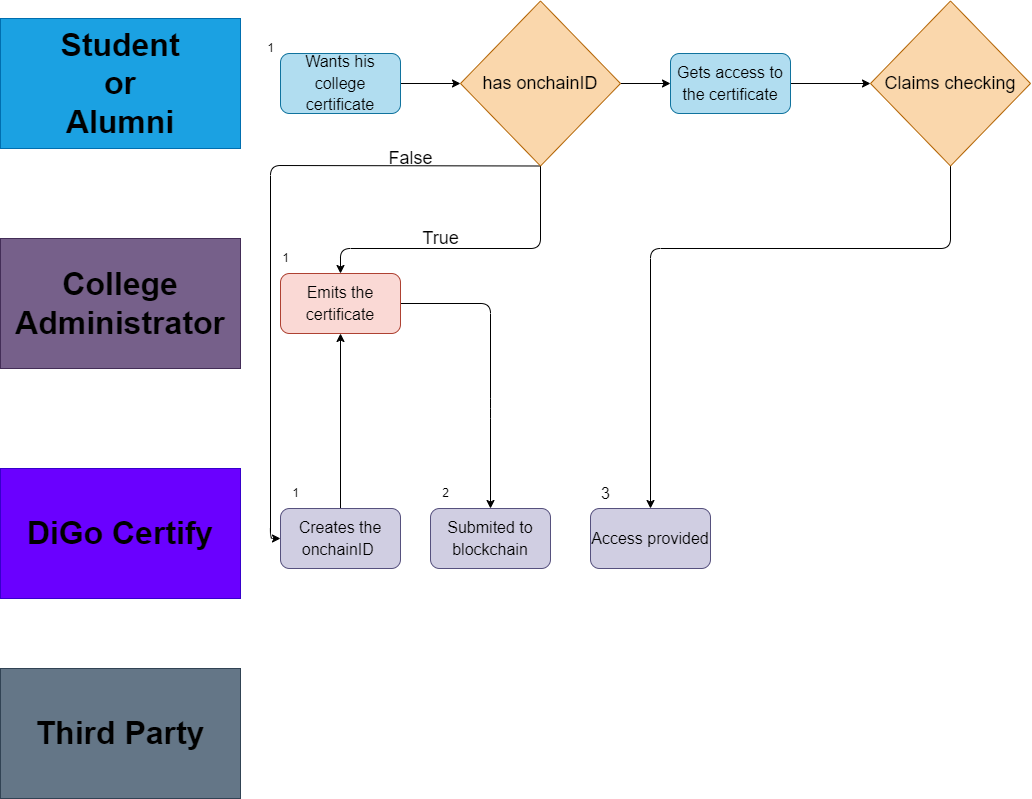
\includegraphics[width=0.6\textwidth, height=0.6\textheight, keepaspectratio]{final-report/assets/certificate-requesting.drawio.png}
    \caption{Use Case 1: Student Registration and Certificate Requesting.}
    \label{fig:use-case-1}
\end{figure}

\begin{itemize}

    \item \textbf{Actors:} Student, College Administrator
    \item \textbf{Description:} A student registers on the mobile application and requests academic certificates from the college administrator.
    \item \textbf{Preconditions:} The student has access to the DiGo Certify platform. The college administrator has access to the platform and the student's academic records.
    \item \textbf{Postconditions:} The student receives the academic certificates and stores them on the blockchain.
    \item \textbf{Main Flow:}
    \item 1. The student downloads the \texttt{DiGo Certify} mobile application from the app store.
    \item 2. The student registers himself using their email address and connecting a wallet to the application.
    \item 3. The student requests academic certificates from the college administrator.
    \item 4. The college administrator issues the certificates, submitting them to the blockchain and
          emits the claims that will allow the student to access the certificates.
    \item 5. The student receives a notification that the certificates are available for download.
    \item \textbf{Alternative Flow:}
    \item 1.1 The student already has an account on the DiGo Certify platform.
    \item 1.2 The student logs in to their account using their email address.
    \item 1.3 The student requests additional academic certificates from the college administrator.
    \item 1.4 The college administrator issues the new certificates and submits them to the blockchain.
    \item 1.5 The student receives a notification that the certificates are available for download.
    \item \textbf{Exceptions:}
    \item 1. The student enters an invalid email address during registration.
    \item 2. The student fails to register on the application due to an error in the process.
    \item 3. The college administrator does not issue the certificates to the student.
    \item \textbf{Notes:} This use case illustrates the process of student registration and certificate requesting on the mobile application. It emphasizes the importance of secure and transparent interactions between the student and the college administrator, enabled by the blockchain technology.
\end{itemize}

\subsection{Use Case 2: Certificate Validation by an External Entity}

\begin{figure}[H]
    \centering
    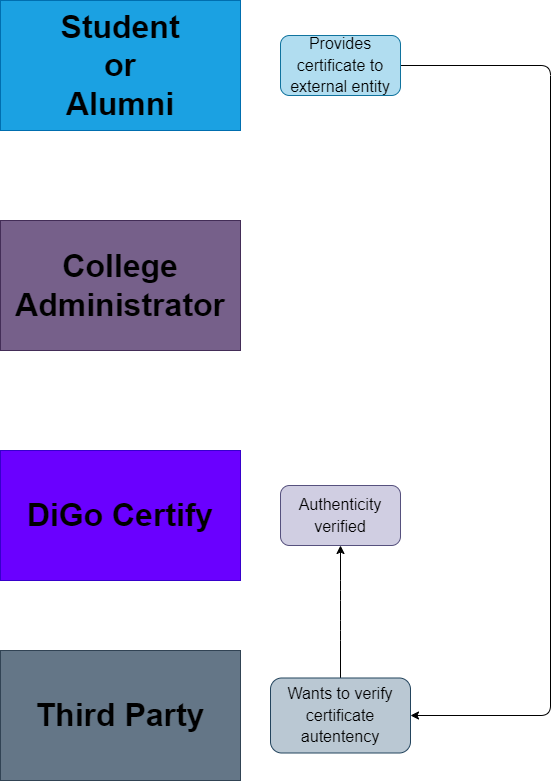
\includegraphics[height=0.6\textwidth, keepaspectratio]{final-report/assets/certificate-validation.drawio.png}
    \caption{Use Case 2: Certificate Verification by an External Entity.}
    \label{fig:use-case-2}
\end{figure}

\begin{itemize}

    \item \textbf{Actors:} External Entity, Student
    \item \textbf{Description:} For the purpose of a job application, an external entity verifies the authenticity of the student's academic certificates on the mobile application.
    \item \textbf{Preconditions:} The employer has access to the \texttt{DiGo Certify} application. The student has shared their certificates with the employer.
    \item \textbf{Postconditions:} The employer confirms the authenticity of the student's certificates and proceeds with the recruitment process.
    \item \textbf{Main Flow:}
    \item 1. The employer does not need to have a wallet to access the application.
    \item 2. The employer scans the QR code or accesses the link shared by the student to view the certificates.
    \item 3. The employer views the student's certificates and verifies their authenticity on the blockchain.
    \item 4. The employer confirms the authenticity of the certificates and proceeds with the recruitment process.
    \item \textbf{Exceptions:}
    \item 1. The employer fails to verify the authenticity of the certificates due to an error in the process.
    \item 2. The employer does not confirm the authenticity of the certificates.
    \item \textbf{Notes:} This use case illustrates the process of certificate verification by an employer on the \texttt{DiGo Certify} mobile application. It emphasizes the importance of transparency and trust in the recruitment process, enabled by the blockchain technology.

\end{itemize}

\subsection{Use Case 3: Student or Alumni requests a change to the certificate}

\begin{figure}[H]
    \centering
    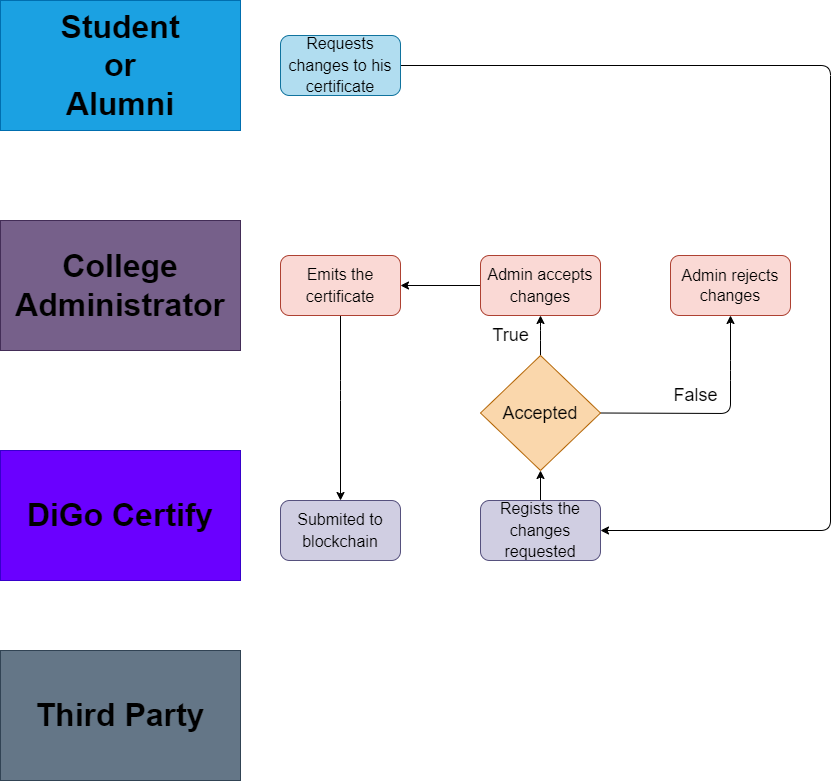
\includegraphics[width=0.6\textwidth, height=0.6\textheight, keepaspectratio]{final-report/assets/certificate-update.drawio.png}
    \caption{Use Case 3: Student or Alumni requests a change to the certificate.}
    \label{fig:use-case-3}
\end{figure}

\begin{itemize}

    \item \textbf{Actors:} Student, College Administrator
    \item \textbf{Description:} A student or alumni requests a change to the academic certificates issued by the college administrator.
    \item \textbf{Preconditions:} The student has access to the DiGo Certify platform. The college administrator has access to the platform and the student's academic records.
    \item \textbf{Postconditions:} The student receives the updated academic certificates and stores them on the blockchain.
    \item \textbf{Main Flow:}
    \item 1. The student logs in to the \texttt{DiGo Certify} mobile application.
    \item 2. The student requests a change to the academic certificates from the college administrator.
    \item 3. The college administrator updates the certificates, submitting them to the blockchain and emits the claims that will allow the student to access the updated certificates.
    \item 4. The student receives a notification that the updated certificates are available for download.
    \item \textbf{Exceptions:}
    \item 1. The student fails to log in to the application due to an error in the process.
    \item 2. The student does not request a change to the academic certificates.
    \item 3. The college administrator does not update the certificates for the student.
    \item \textbf{Notes:} This use case illustrates the process of requesting a change to academic certificates on the mobile application. It emphasizes the importance of maintaining accurate and up-to-date records on the blockchain, enabled by the blockchain technology.

\end{itemize}

\thispagestyle{empty}
\mbox{}
%
% Chapter 4
%
\chapter{Solution Architecture}\label{chap:architecture}

The present chapter covers the system's components, their interactions, and the underlying technologies used to implement the solution. The architecture is designed to ensure data integrity, security, and scalability while providing a seamless user experience. We will cover the concept of a multiplatform application, how it functions, the various solutions available, and a detailed discussion of the chosen technology stack, specifically React Native with the Expo\cite{Expo} platform.

\section{Architecture Overview}\label{sec:architecture-overview}

The architecture of the \texttt{DiGo Certify} system is designed to be modular, scalable, and secure. The system~\ref{fig:architecture-overview} is divided into two main layers: the mobile application layer and the fully distributed layer. Each layer has specific responsibilities and interacts with the others to deliver the desired functionality.

\subsubsection{Mobile Application Layer}

The mobile application layer consists of the DiGo Certify application, which is built using React Native and Expo. This application is responsible for the user interface and handles interactions with the end-users. The choice of React Native ensures that the application is cross-platform, providing a seamless experience on both iOS and Android devices. The application allows users to register, authenticate, and manage their certificates. It communicates with the distributed layer to store and validate these certificates on the Ethereum blockchain.

\subsubsection{Fully Distributed Layer}

The fully distributed layer is implemented using the Ethereum blockchain. It consists of smart contracts written in Solidity, which handle the storage and validation of academic certificates. This layer leverages the security and immutability of the blockchain to ensure the integrity of the certificates. The interaction between the mobile application and the blockchain is facilitated by a provider, such as Hardhat, which helps in deploying and managing the smart contracts.

\paragraph{}
Below is a high-level diagram of the DiGo Certify architecture:

\begin{figure}[H]
    \centering
    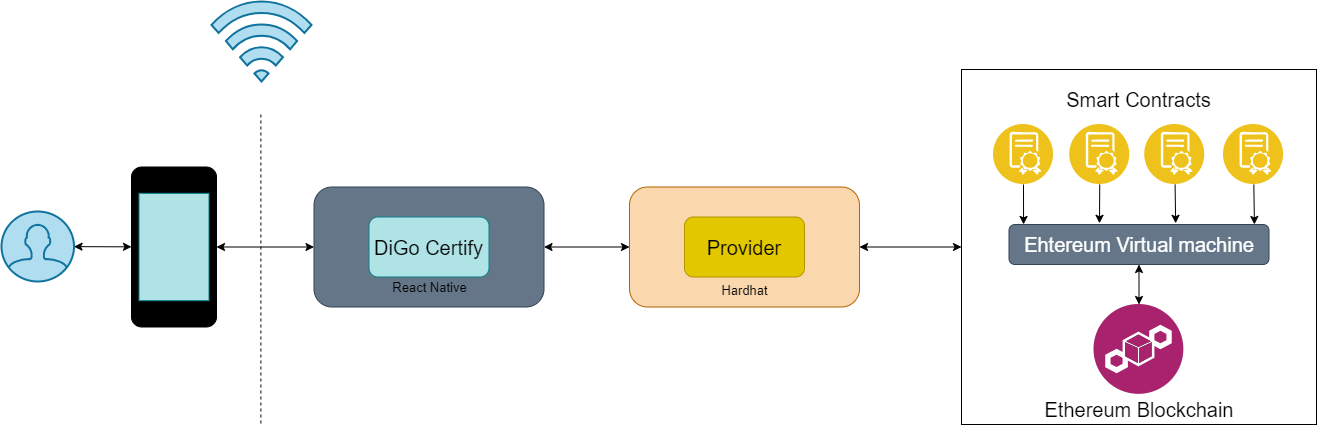
\includegraphics[width=1\textwidth]{../diagrams/architecture-overview.drawio.png}
    \caption{Architecture Overview Diagram (inspired by~\cite{geeksforgeeks-dApps}).}
    \label{fig:architecture-overview}
\end{figure}

\section{Fully Distributed Environment}\label{sec:fully-distributed-environment}

The fully distributed environment of the DiGo Certify system leverages blockchain technology to create a secure, decentralized, and transparent platform for managing academic certificates. By using the Ethereum blockchain, the system ensures that certificates are immutable and verifiable by any third party, thereby eliminating the risk of fraud and enhancing trust in the certification process.

\subsection{Smart Contracts on Ethereum}

At the core of the distributed environment~\ref{fig:architecture-overview} are the smart contracts deployed on the Ethereum blockchain. Smart contracts are self-executing contracts with the terms of the agreement directly written into code. In the context of DiGo Certify, these smart contracts handle the issuance, validation, and storage of academic certificates. Each certificate is represented as a unique digital asset on the blockchain, and its authenticity can be easily verified by checking the blockchain records.

The smart contracts are written in Solidity, a statically-typed programming language designed for developing smart contracts that run on the Ethereum Virtual Machine (EVM). The key functions of these smart contracts include:

\begin{itemize}
    \item \textbf{Certificate Issuance:} This function allows authorized entities, such as educational institutions, to issue certificates to students. The institution submits a transaction to the smart contract, including details such as the student’s name, course, and date of completion. Upon verification, the smart contract records the certificate on the blockchain.

    \item \textbf{Certificate Validation:} This function enables third parties, such as employers, to verify the authenticity of a certificate. By querying the blockchain, they can confirm that the certificate was indeed issued by a legitimate institution and has not been altered.

    \item \textbf{Certificate Storage:} Certificates are stored in a decentralized manner on the blockchain. This ensures that they are \textit{tamper-proof} (i.e., they cannot be altered or manipulated) and can be accessed by anyone with the appropriate permissions.

\end{itemize}

\subsection{Ethereum Virtual Machine (EVM)}

The Ethereum Virtual Machine (EVM) is a decentralized computing environment that executes smart contracts on the Ethereum network. The EVM ensures that the execution of smart contracts is consistent and secure across all nodes in the network\cite{EVM}. This decentralized nature of the EVM makes it highly resistant to hacking and fraud, as any attempt to alter a certificate would require the attacker to gain control of a majority of the network’s computing power, which is practically impossible. Once a certificate is recorded on the blockchain, it cannot be altered or deleted, ensuring that the certificates remain trustworthy and verifiable indefinitely. Additionally, all transactions on the Ethereum blockchain are publicly accessible, providing a transparent record of certificate issuance and validation, which enhances trust in the certification process.

\subsection{Provider (Hardhat)}

Hardhat is a comprehensive development environment for Ethereum software, providing an array of tools for compiling contracts, running tests, and deploying them to the blockchain. It significantly simplifies the development and deployment process, making it easier to manage the smart contracts that underpin the DiGo Certify system.

During the development phase, Hardhat is used to compile Solidity code into bytecode that can be executed by the Ethereum Virtual Machine (EVM). It allows developers to write and run tests, ensuring that smart contracts behave as expected. Hardhat also provides scripts for deploying smart contracts to the Ethereum network, making the deployment process straightforward and repeatable.

In addition to its development capabilities, Hardhat also plays a role in facilitating the interaction between the mobile application and the blockchain during the execution phase. This ensures smooth and secure communication between the components of the DiGo Certify system. Although primarily a development tool, Hardhat's robust features and integration capabilities make it useful throughout the lifecycle of the smart contracts.

In the context of the DiGo Certify system, Hardhat serves as a development and deployment environment, while also supporting interaction with the blockchain during execution. It's important to note that other tools and services, such as Infura or Alchemy, can be used as blockchain providers during execution. These services offer additional capabilities, such as scalable node infrastructure and advanced monitoring, but in our implementation, Hardhat has proven sufficient for both development and interaction purposes.

\subsection{Security}

Security and scalability are critical considerations in the design of the DiGo Certify system. The Ethereum blockchain’s inherent security features, such as its decentralized consensus mechanism and cryptographic algorithms, providing a robust foundation for secure certificate management. Additionally, the use of smart contracts ensures that certificate issuance and validation processes are automated and tamper-proof\cite{Wood2014}.

\section{Mobile Application}\label{sec:mobile-application}

\subsection{Multiplatform Application}\label{sec:multiplatform-application}

A multiplatform application is designed to run seamlessly on multiple operating systems, such as iOS and Android, using a single codebase. This approach significantly reduces development time and costs while ensuring a consistent user experience across different devices. The core idea is to write the code once and deploy it across multiple platforms, which is particularly beneficial for applications that need to reach a broad audience.

\subsubsection{Functionality and Operation}

Multiplatform applications leverage frameworks that provide tools and libraries to facilitate cross-platform development. These frameworks abstract away the differences between the various platforms, allowing developers to focus on building features rather than dealing with platform-specific nuances. The primary goal is to achieve native-like performance and look-and-feel while maintaining a shared codebase.

\subsubsection{Available Solutions}

Several frameworks are available for developing multiplatform applications, each with its own set of features and trade-offs. The most notable ones include:

\begin{itemize}
    \item React Native\cite{ReactNativeBook}
    \item Flutter\cite{Flutter}
    \item Kotlin Multiplatform Mobile (KMP)\cite{KMP}
\end{itemize}

\subsubsection{React Native}

React Native is a popular open-source framework developed by Facebook. It allows developers to build mobile applications using JavaScript and React, a widely-used library for building user interfaces. React Native bridges the gap between web and mobile development by enabling code reuse across platforms while providing near-native performance\cite{ReactNativeBook}.

\paragraph{Key Features:}

\begin{itemize}
    \item \textbf{Component-Based Architecture:} Enables modular and maintainable code.
    \item \textbf{Hot Reloading:} Allows developers to see changes in real-time without recompiling the entire application.
    \item \textbf{Rich Ecosystem:} A vast collection of libraries and tools that streamline development.
    \item \textbf{Community Support:} Extensive community contributions and support.
\end{itemize}

\subsubsection{Flutter}

Flutter, developed by Google, is another powerful framework for building natively compiled applications for mobile, web, and desktop from a single codebase. It uses the Dart programming language and provides a rich set of pre-designed widgets to create highly customizable interfaces\cite{Flutter}.

\paragraph{Key Features:}

\begin{itemize}
    \item \textbf{Hot Reload:} Similar to React Native's hot reloading, enabling quick iterations.
    \item \textbf{Expressive UIs:} Rich set of customizable widgets.
    \item \textbf{Performance:} Compiled directly to native code, which can lead to better performance.
\end{itemize}

\subsubsection{Kotlin Multiplatform Mobile (KMP)}

KMP, developed by JetBrains, allows developers to use Kotlin for developing iOS and Android applications. It focuses on sharing code, particularly business logic, while allowing platform-specific code where necessary\cite{KMP}.

\paragraph{Key Features:}

\begin{itemize}
    \item \textbf{Code Sharing:} Share common code across platforms while writing platform-specific code when needed.
    \item \textbf{Native Performance:} Utilizes native components and performance optimizations.
\end{itemize}

\subsection{Chosen Solution: React Native with Expo}

For the \texttt{DiGO Certify} application, we chose React Native with the \texttt{Expo} platform. This decision was influenced by several factors, including our team's familiarity with JavaScript and React, the maturity and stability of the React Native ecosystem, and the added benefits provided by Expo\cite{Expo}.

To make an informed decision, we compared several frameworks, including Flutter and Kotlin, based on various parameters~\ref{tab:comparison}.

\begin{table}[h]
    \centering
    \label{tab:comparison}
    \caption{Comparison of Flutter, React Native, and Kotlin.\cite{RNvsFluttervsKMP}}
    \begin{tabular}{|p{2.5cm}|p{4cm}|p{4cm}|p{4cm}|}
        \hline
        \textbf{Parameter}         & \textbf{Flutter}                           & \textbf{React Native}                             & \textbf{Kotlin}                                                        \\ \hline
        \textbf{Ease of Coding}    & Widget-based, reactive framework (Dart)    & JSX and JavaScript, component-based (React)       & Concise, expressive, reduces boilerplate (Kotlin)                      \\ \hline
        \textbf{Scalability}       & Good scalability, reactive architecture    & Scales well, may need native modules              & Excellent scalability, especially for large codebases                  \\ \hline
        \textbf{Performance}       & High performance, compiled language (Dart) & Near-native performance, native modules if needed & Efficient performance, native language for Android                     \\ \hline
        \textbf{Learning Curve}    & Moderate, widget-based approach            & Relatively easy for JavaScript developers         & Moderate, especially for those familiar with Java                      \\ \hline
        \textbf{Popularity}        & Growing rapidly, gaining popularity        & Widely adopted, mature, and well-established      & Highly popular for Android development                                 \\ \hline
        \textbf{Stability}         & Stable, regular updates and improvements   & Stable, backed by Facebook and active community   & Stable, regular updates and improvements                               \\ \hline
        \textbf{Types of App Dev}  & Cross-platform focus for consistent UI     & Cross-platform, leverages JavaScript expertise    & Primarily for native Android; Kotlin Multi Platform for cross-platform \\ \hline
        \textbf{Community Support} & Growing community support                  & Large and active community support                & Strong support, especially in the Android community                    \\ \hline
    \end{tabular}
\end{table}


React Native’s component-based architecture aligns well with our need for a modular and maintainable codebase. Our team’s existing knowledge of JavaScript and React significantly reduced the learning curve, allowing us to quickly become productive and focus on delivering features. Compared to Flutter and Kotlin, React Native's learning curve is relatively easy for JavaScript developers, while Flutter requires learning Dart, and Kotlin, despite being expressive and reducing boilerplate, may be more moderate for developers familiar with Java.

In terms of performance, React Native provides near-native performance, ensuring that our application runs smoothly on both iOS and Android\cite{react-native-performance}. This is similar to Flutter~\ref{tab:comparison}, which offers high performance through its compiled language, Dart, and Kotlin, which provides efficient performance for native Android development. However, React Native can scale well with the potential need for native modules, providing flexibility in development.

The framework’s rich ecosystem of libraries and tools further accelerated our development process, providing pre-built components and solutions that we could easily integrate into our application. The extensive community support for React Native ensured that we had access to numerous resources, tutorials, and third-party libraries, which proved invaluable during the development process. This support network allowed us to quickly troubleshoot issues and implement best practices, contributing to a more efficient development cycle. While Flutter's community is rapidly growing, React Native's community is already large, mature, and well-established, and Kotlin also enjoys strong support, especially in the Android community.

Expo enhances React Native by offering a suite of tools and services that simplify development\cite{Expo}. With Expo, we benefit from an integrated environment for developing, building, and deploying React Native applications. The platform’s managed workflow handles many of the complexities of building and deploying mobile applications, allowing us to focus on developing features rather than dealing with infrastructure. Expo’s easy setup and configuration process streamlined our project initialization, while its over-the-air update capability enables us to push updates to users without requiring a full app store review process.

The development workflow for DiGo Certify using React Native and Expo involves several key steps. Initially, we set up the project with Expo CLI, which provides a streamlined setup process and essential tools. We then focused on building the application UI using React Native’s component-based approach. This method allows us to create reusable UI elements that help maintain consistency and simplify development.

For integrating blockchain functionality, we implemented smart contracts in Solidity and connected them with the React Native application through ethers.js. This integration enables secure interactions with the Ethereum blockchain, allowing for the storage and validation of academic certificates.

Testing and debugging are facilitated by Expo’s built-in tools, which allow us to test the application on various devices and simulators. This ensures that our application performs well across different platforms and devices. Finally, Expo simplifies the deployment process with its build and publish services, allowing us to distribute the application through app stores seamlessly.

In summary, the choice of React Native with Expo for DiGo Certify provides a robust, efficient, and scalable solution for developing a secure and user-friendly multiplatform application. This architecture leverages modern technologies to meet the needs of our diverse user base, ensuring a high-quality user experience across all supported devices.

\section{Proposed Model}

\subsection{Certificate Issuance}

Initially, a student or alumni requests a certificate from the OnchainID~\cite{ONCHAINID} system. The system checks whether the requester has an existing OnchainID. If it exists, the system proceeds to verify the associated claims and sends the certificate to the DiGo Certify application. The application then submits the certificate to the blockchain for validation and secure storage. Once the certificate is successfully submitted, it is delivered back to the student or alumni. In cases where the OnchainID does not exist, the system initiates the creation of a new identifier. This involves sending a certificate emission request to the Admin for approval. Upon receiving the request, the Admin emits the certificate and submits it to the blockchain. After the submission, the certificate is sent back to the OnchainID system, which verifies the claims and delivers the certificate to the student or alumni. This process ensures that all issued certificates are securely stored on the blockchain, providing a tamper-proof and verifiable record of the certification.

\begin{figure}[H]
    \centering
    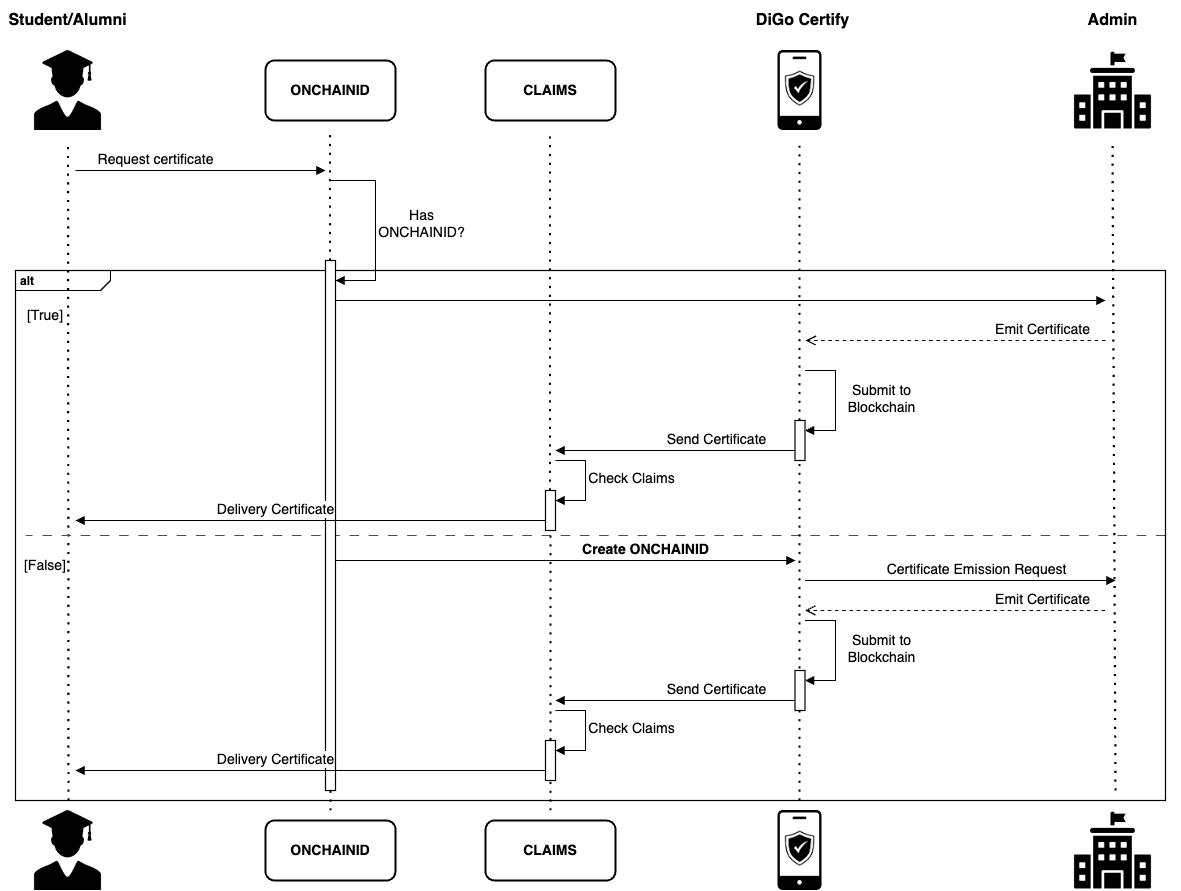
\includegraphics[width=0.6\textwidth]{../diagrams/certificate-request-diagram-sequence.png}
    \caption{Certificate Issuance.}
    \label{fig:certificate-issuance}
\end{figure}

\subsection{Requesting and Approving changes on a certificate}

The process begins with the student or alumni initiating a request for changes to their certificate. The DiGo Certify application then submits the modified certificate to the blockchain for validation. Upon processing the transaction, the blockchain provides a confirmation of the changes. This confirmation is sent back to the student or alumni, notifying them of the acceptance or denial of the requested changes. Concurrently, the Admin is notified of the requested changes. If the changes are approved, the Admin emits a new certificate with the modifications and submits it to the blockchain. The modified certificate is processed by the blockchain, completing the transaction. This process allows for the secure and transparent modification of certificates, ensuring that any changes are recorded on the blockchain and are verifiable by all parties involved.

\begin{figure}[H]
    \centering
    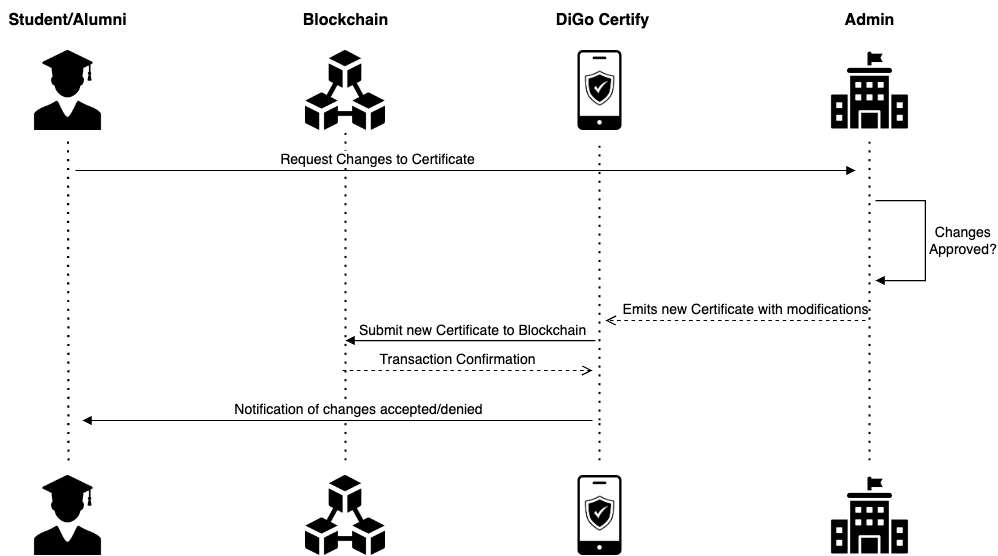
\includegraphics[width=0.6\textwidth]{../diagrams/certificate-update-diagram-sequence.png}
    \caption{Certificate update request.}
    \label{fig:certificate-update}
\end{figure}

\subsection{Certificate Validation}

When a student or alumni first provides their certificate to a third party who needs to verify its authenticity. The third party then initiates an authentication request to the DiGo application. Upon receiving the request, the DiGo verifies the certificate's authenticity by checking its records against the blockchain. This verification process ensures that the certificate has not been tampered with and is indeed issued by a recognized authority. Once the verification is complete, the DiGo Certify application confirms the authenticity of the certificate back to the third party. Subsequently, the third party can confidently rely on the certificate's validity, and the student or alumni is informed of the successful verification. This process underscores the importance of blockchain in maintaining the integrity and trustworthiness of academic certificates, ensuring that any third party can independently confirm their authenticity without relying solely on the issuing institution.

\begin{figure}[H]
    \centering
    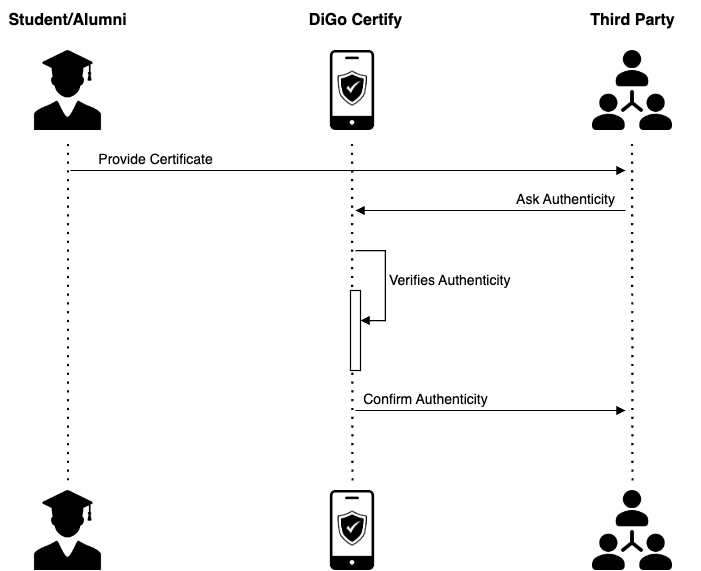
\includegraphics[width=0.6\textwidth]{../diagrams/certificate-validation-diagram-sequence.drawio.png}
    \caption{Certificate update request.}
    \label{fig:certificate-validation}
\end{figure}

\newpage
\thispagestyle{empty}
\mbox{}
%
% Chapter 5
%
\chapter{Implementation}\label{chap:implementation}

The present chapter, will be developed and expanded upon in subsequent phases of the project, providing detailed insights into the implementation process and technical aspects of the solution.

\section{Mobile Application}\label{sec:mobile-application-implementation}

The mobile application layer, as previously mentioned at Section \ref*{sec:mobile-application}, is responsible for providing the user interface and interaction with the user. The application is developed using React Native\cite{ReactNativeBook} and Javascript\cite{Javascript} along with the Expo platform, which allows for the development of cross-platform applications, with a single codebase. The application is divided into several components, each responsible for a specific part of the application. The structure of the application is as follows:

\begin{itemize}
    \item \textbf{App} - Contains the main application files and folders such as authentication, navigation tabs, and initial screens.
    \item \textbf{Components} - Houses reusable UI components used throughout the application.
    \item \textbf{Assets} - Contains the images, icons, and colors used in the application.
    \item \textbf{Services} - Includes utility functions and services that handle tasks such as API calls and interaction with smart contracts.
\end{itemize}

\subsection{Application Structure and Design Philosophy}

The DiGo Certify mobile application is built on the principles of modularity, scalability, and maintainability. These principles guide the design and organization of the application, ensuring that each component is independent, reusable, and easy to maintain. The application leverages the Expo Router\cite{Expo-Router} for file-based routing, which provides a straightforward and efficient way to manage navigation within the app.

\subsubsection{File-Based Routing~\cite{Expo-Router-File-Based-Routing}}

File-based routing is a core feature of the Expo Router, allowing routes to be defined based on the file structure within the \texttt{app} directory. This approach simplifies the process of adding new routes and ensures a consistent and intuitive navigation structure. Each file or directory within the \texttt{app} directory represents a distinct route in the application.

For instance, the file \texttt{app/index.jsx} corresponds to the root route ("/"), and any additional files or nested directories create corresponding nested routes. This method provides a clear and organized way to manage the application's navigation, making it easy to understand and extend.

\begin{itemize}
    \item \textbf{Example:} Creating a new route is as simple as adding a new file. For example, adding a \texttt{details.jsx} file inside the \texttt{app} directory will create a new route accessible at "/details".
\end{itemize}

The \texttt{\_layout.jsx} file plays a crucial role in defining shared UI elements such as headers and footers that persist across different routes. This file acts as the root layout, ensuring a consistent look and feel throughout the application.

\subsubsection{Dynamic Routing}

Dynamic routing in Expo Router allows for more flexible navigation patterns by incorporating dynamic segments in the URL paths. This is particularly useful for routes that depend on parameters, such as user profiles or specific certificate details.

Dynamic segments are defined using square brackets in the file names. For example, a file named \texttt{[id].jsx} within a directory will match any URL segment, treating it as a variable. This allows the application to handle a wide range of dynamic routes efficiently.

\begin{itemize}
    \item \textbf{Example:} A route defined by \texttt{details/[id].jsx} can handle URLs like "/details/1" or "/details/2", where the segment after "/details/" is dynamic and can vary.
\end{itemize}

Expo Router's \texttt{Link} component is used to navigate between routes. It works similarly to the HTML \texttt{<a>} tag, using the \texttt{href} attribute to specify the target route. This component simplifies the process of linking different parts of the application, making the navigation seamless and intuitive.

\begin{itemize}
    \item \textbf{Example:} Using the \texttt{Link} component to navigate to a dynamic route can be done by passing the dynamic segment as a parameter: \texttt{<Link href="/details/1">View Details</Link>}.
\end{itemize}

\subsubsection{Advantages of File-Based and Dynamic Routing}

The combination of file-based and dynamic routing in Expo Router offers several advantages:

\begin{itemize}
    \item \textbf{Simplicity:} The file-based approach reduces the complexity of defining and managing routes, aligning with the project's philosophy of simplicity and maintainability.
    \item \textbf{Scalability:} As the application grows, new routes can be added easily by creating new files, making the application scalable without requiring significant changes to the existing structure.
    \item \textbf{Flexibility:} Dynamic routing allows for handling a wide range of navigation scenarios, providing the flexibility needed to support complex user interactions.
    \item \textbf{Consistency:} The use of layout files ensures that shared UI elements are consistently applied across different routes, providing a cohesive user experience.
\end{itemize}

In summary, the DiGo Certify application leverages the power of Expo Router's file-based and dynamic routing to create a robust, scalable, and maintainable navigation structure. This approach aligns with the overall design philosophy of the project, ensuring that the application is easy to extend, manage, and use.

\subsection{App Directory}

The \texttt{app} directory is the core of the application, containing the main screens and navigation setup. It is organized as follows:

\begin{itemize}
    \item \textbf{auth} - Manages the authentication flow.
    \item \textbf{tabs} - Handles the tab-based navigation within the application, such as Home, Profile, and Settings. This provides an intuitive way for users to navigate through different sections of the app.
    \item \textbf{initial-screen} - Contains the initial screen components displayed when the application is first launched. This includes splash screens and welcome messages that enhance the user onboarding experience.
    \item \textbf{\_layout.jsx} - Defines the layout structure of the application, including the header and footer components. This ensures a consistent look and feel across different screens.
    \item \textbf{emission.jsx} - Manages the certificate emission process, allowing administrators to issue new certificates. This is a critical component for the functionality of the DiGo Certify app.
    \item \textbf{index.jsx} - The entry point for the app directory, setting up the initial routing and navigation. This file integrates all the major components and initiates the application.
\end{itemize}

\subsection{Services Directory}

The services in the DiGo Certify frontend application play a crucial role in facilitating communication with the Ethereum blockchain and backend systems. Each blockchain interaction and backend microservice has a corresponding service in the frontend application, acting as a namespace that contains functions responsible for handling specific requests. These functions are asynchronous and return promises that resolve to the responses from these requests.

To interact with the Ethereum blockchain, the application utilizes the \texttt{ethers.js} library~\cite{ethers}, which provides a comprehensive set of tools for creating wallets, signing transactions, deploying smart contracts, and interacting with them. This library is chosen for its simplicity, robustness, and extensive documentation, making it ideal for handling blockchain operations within the application.

The \texttt{services} directory includes utility functions and services that handle tasks such as API calls, smart contract interactions, authentication processes, and secure storage. This directory is vital for maintaining clean and modular code, ensuring that the application's logic is well-organized and easily maintainable.

\subsubsection{Blockchain Services}

The \texttt{ethereum} directory within \texttt{services} handles interaction with the Ethereum blockchain, including smart contract calls. This service abstracts the complexity of blockchain interactions and provides simple methods for the application to use. Functions within this service manage tasks such as deploying contracts, invoking smart contract methods, and listening for events emitted by the contracts.

\subsubsection{Secure Storage}

Secure storage is a critical aspect of managing sensitive information within the application. The \texttt{storage.js} file within the \texttt{storage} directory leverages Expo's Secure Store~\cite{Expo-Secure-Store} to securely store sensitive data on the device. Expo Secure Store is a key-value storage system that encrypts data at rest, ensuring that sensitive information such as private keys and authentication tokens are stored securely.

\begin{itemize}
    \item \textbf{Expo Secure Store:} Provides a secure way to store sensitive key-value pairs on the device. It encrypts data at rest, making it a suitable choice for storing private keys and authentication tokens.
\end{itemize}

\subsubsection{WalletConnect Integration}

WalletConnect~\cite{Wallet-Connect} is integrated into the application to facilitate secure and user-friendly connections to Ethereum wallets. The \texttt{wallet-connect.js} file within the \texttt{web3} directory manages the WalletConnect integration. This service enables users to connect their Ethereum wallets to the DiGo Certify application, allowing for seamless interaction with the blockchain.

\begin{itemize}
    \item \textbf{WalletConnect:} A protocol that enables secure connections between the application and Ethereum wallets. It allows users to interact with the blockchain using their preferred wallet, enhancing the user experience and security.
\end{itemize}

\subsection{User Interface}

The user interface (UI) design of the DiGo Certify application focuses on simplicity, usability, and accessibility. The design principles are aimed at providing a seamless user experience that caters to the needs of all users, including students, alumni, and administrators.
The user journey diagram in Figure \ref{fig:user-journey} illustrates the key interactions and flows within the application, highlighting the various paths users can take to achieve their goals.

\begin{figure}[H]
    \centering
    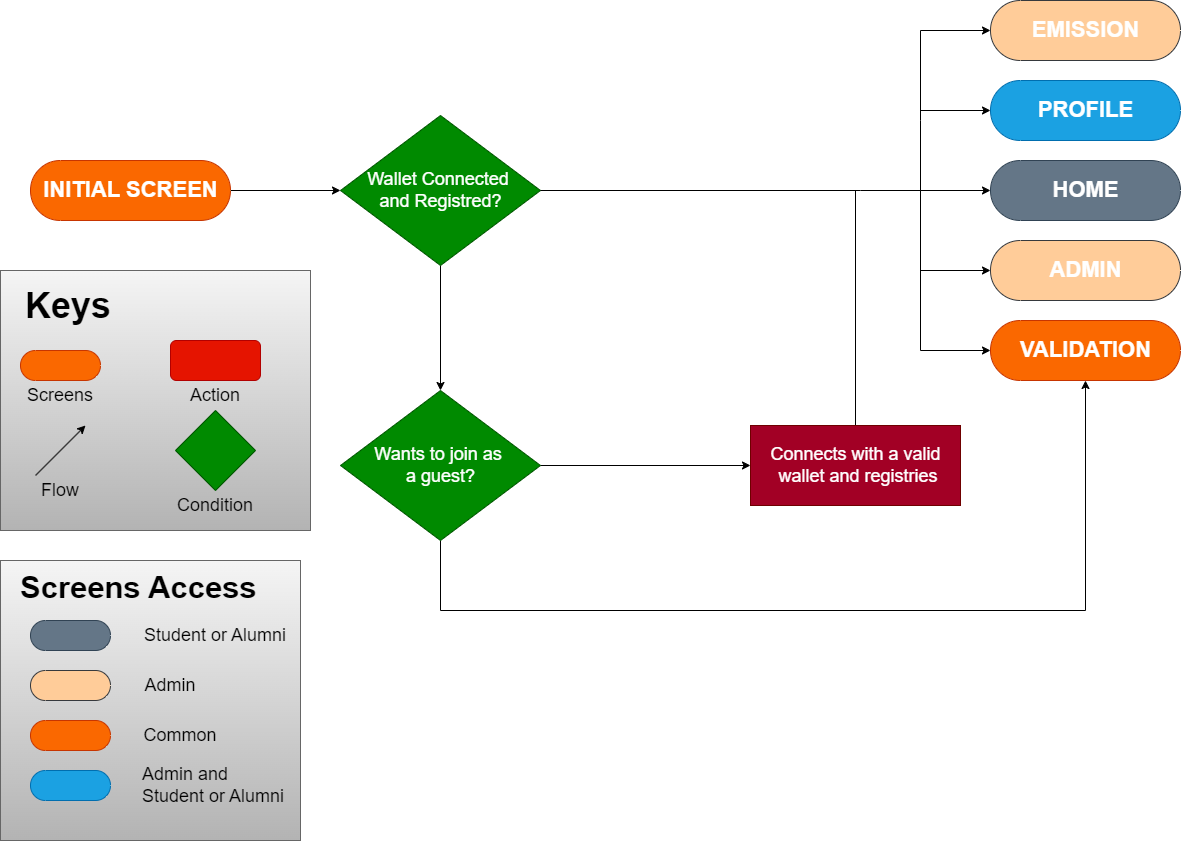
\includegraphics[width=0.7\textwidth]{final-report/assets/app-flow.drawio.png}
    \caption{User Journey Diagram}
    \label{fig:user-journey}
\end{figure}

\section{Interaction with Smart Contracts}\label{sec:interaction-with-smart-contracts}
\paragraph{}

In this section we will briefly introduce the interaction between the DiGo Certify App and the Ethereum blockchain through smart contracts, outlining the importance of this interaction for the functionality of the application.

\subsection{Libraries and Tools for Blockhain Interaction}\label{subsec:utilizing-libraries-and-tools}
\paragraph{}

DiGo Certify App interacts with the smart contracts deployed on the Ethereum blockchain. The smart contracts are responsible for all the business logic of the application.
To make this interaction possible we used the \textit{ethers~\cite{ethers}} library which provides a set of tools to interact with the Ethereum blockchain, such as creating wallets, signing transactions, deploying smart contracts, and interacting with them~\cite{ethersDocs}.

The contracts that need to be present in the blockchain are deployed using \textit{Hardhat~\cite{hardhat}} that is a powerful Ethereum development environment that offers a comprehensive suite of tools for building, testing, and deploying smart contracts.
It provides an efficient and developer-friendly framework, streamlining the complex processes involved in Ethereum development. It offers a variety of features that are essential for modern blockchain development, such as
flexible plugin system~\cite{hardhatPlugins}, built-in tasks and scripts, hardhat network~\cite{hardhatNetwork}, smart contract debugging~\cite{hardhatDebug} and a good integration with the ethers library~\cite{hardhatWithEthers}.

\subsection{Managing Identities and Certificates}\label{subsec:managing-identities-and-certificates}
\paragraph{}

In our implementation, we leverage the \textbf{OnchainID~\cite{ONCHAINID}} and \textbf{Tokens for Regulated EXchanges~\cite{trexPurposeAndArchitecture}} contracts to manage identities, institutions, and certificates.
OnchainID is a blockchain-based identity system that identifies individuals and organisations, allowing them to enforce compliance and access digital assets~\cite{onchainidPruposalAndArchitecture}.
Their address is a unique identifier that can safely be used by a service provider to identify their owner and provide access to their services. Identities are smart contracts that support the ERC734: Key Manager~\cite{Vogelsteller_2017_key_manager} and ERC735: Key Holder~\cite{Vogelsteller_2017} standards, which define the structure of claims and keys, respectively.
The tools provided by OnchainID facilitate a secure, efficient, and scalable system for handling academic certificate emission onto the blockchain.
The OnchainID suite provides a comprehensive identity framework, ensuring that each participant in the ecosystem has a unique and verifiable identity
that can be used to issue, verify, and store academic credentials.
To simplify the deployment and management of identities, we use the \textit{IdentityFactory} contract from the OnchainID suite that follows the Factory pattern~\cite{harmes2008factory}, a design pattern recommended in the OnchainID documentation, which simplifies the creation and management of multiple instances of identities.
Every contract needed for the OnchainID is provided by a framework with the plugin \textbf{@onchain-id/identity-sdk} that was developed by the OnchainID team and provides easily import of the contracts.
On the other hand, T-REX does not provide a similar framework, so we had to import our own contracts to deploy the T-REX suite automated by the \textbf{deployTrexSuite} script.

The T-REX is a suite of blockchain-based solutions to issue and manage compliant security tokens on a distributed IT infrastructure. T-REX is Tokeny's implementation of the ERC3643 token standard used to manage institutions that issue certificates and the certificates themselves.
This suite provides a robust framework for handling the issuance and verification of academic credentials.
Similar to OnchainID, the T-REX suite utilizes the Factory pattern for creating and managing certificate-issuing contracts and also
use the Proxy pattern~\cite{harmes2008proxy} to create a proxy contract that acts as a gateway to the certificate-issuing contracts, allowing for upgrades to the certificate management logic without disrupting existing data.
This ensures that the system remains adaptable to future changes and improvements.
The T-REX suite includes registries for trusted issuers that work similarly as a Whitelist, allowing that only verified institutions that are present in the registry can issue certificates. This registry is crucial for maintaining the system's integrity, as it prevents unauthorized entities from issuing fraudulent certificates.

\subsection{Contract Interaction Setup}\label{subsec:interacting-with-the-contracts}
\paragraph{}

To be able to interact with the contracts, hardhat compile and stores the contract's ABI (Application Binary Interface) and the contract's address in a JSON file that is generated before launching the application by the auxiliary script \textbf{install.sh}.
The ABI is a JSON representation of the contract's interface, which includes the functions, events, and variables of the contract. The address is the location of the contract on the blockchain.

After the contracts are deployed, the application interact with them using the \textit{ethers.js} library and a set of helper functions that were created to facilitate the interaction with the contracts (e.g \textbf{getContractAt}, \textbf{getWallet}\dots).
These functions are located in the \textit{utils} folder of the ethereum services and are imported in the necessary components.

\section{Smart Contracts}\label{sec:smart-contracts-implementation}
\paragraph{}

In this section we offer a thorough description of the implementation of the most important smart contracts used in the system. For more detailed information about the app architecture, consult Section~\ref{sec:fully-distributed-environment}.
The core of the services provided by the DiGo Certify App is the management of digital identities and certificates on the blockchain and they are implemented in the \textbf{ethereum} folder of the project with the following structure:

\begin{itemize}
    \item \textbf{contracts}: Contains the smart contracts deployed on the blockchain.
    \item \textbf{scripts}: Houses functions responsible for automating blockchain operations, such as contract deployment and interaction.
          \subitem\textbf{identities}: Functions related to the management of digital identities.
          \subitem\textbf{claimIssuer}: Functions pertaining to institutions that issue certificates.
          \subitem\textbf{claims}: Functions associated with the issuance of certificates.
          \subitem\textbf{suites}: Functions for deploying the OnchainID and T-REX suites.
          \subitem\textbf{utils}: Helper functions utilized throughout the application.
    \item \textbf{test}: Includes test scripts and cases validating the functionality of contracts and scripts.
\end{itemize}

\subsection{Institution Creation}\label{subsec:creating-institutions}
\paragraph{}

In this section, we discuss the process of creating institutions, known within the DiGo Certify App as Claim Issuers, on the Ethereum blockchain.
Claim Issuers are entities that have the authority to issue certificates to students and alumni. The creation of Claim Issuers is a crucial step in the certification validation process, as it ensures that only verified institutions can issue certificates.
The Claim Issuer creation process is automated through the use of the \textbf{deployClaimIssuer} function, which is responsible for deploying a new Claim Issuer contract associated with a specified wallet address.

The function begins by deploying into the blockchain a new Claim Issuer contract for the specified address and waits until the block is mined in order to retrieve the deployed contract instance.
After the Claim Issuer contract deployment, we access the \textbf{TrustedIssuerRegistry} contract, which is the Whitelist of trusted issuers, and add the new Claim Issuer to the registry making the new
Claim Issuer a trusted entity that can issue certificates. This is done by calling the \textbf{addTrustedIssuer} function of the TrustedIssuerRegistry contract, which requires the Claim Issuer address and a predefined list of permitted claim topics. See with more detail in Section~\ref{subsubsec:understanding-claims-and-certificates}.
After being in the whitelist, the institution self assign his institution code for future identification and reference within the application.
In the end the claim issuer contract address, abi, institution code and both public and private keys are stored in the configuration file.

This entire process is managed through a shell script, accessible exclusively to the owner of the DiGo Certify App. This measure ensures that only authorized personnel can initiate and oversee the creation of new Claim Issuers, maintaining the integrity and security of the certification issuance framework.

\subsection{Identity Creation}\label{subsec:creating-identities}
\paragraph{}

The first step in the process of the certification validation process is the creation of a student identity. After the registration process at the beginning of the app, the student's identity is created on the blockchain.
This is done by calling the \textbf{deployIdentity} function that contains all the necessary logic to create a new identity. The primary objective of this function is to automate the process of deploying a new identity contract associated with a specified wallet address.
It begins by validating inputs such as the wallet address and a unique cryptographic salt used for identity creation, ensuring that the identity is unique. This is a read-write operation
that requires to be signed by the owner private key. Upon successful deployment the function monitors the blockchain for relevant events, such as \textbf{WalletLinked} to confirm the identity creation.

Once created the function retrieves the deployed identity contract instance that allows subsequent interactions and operations with the newly created identity contract.

\subsection{Asking for a Certificate}\label{subsec:asking-for-a-certificate}
\paragraph{}

After having a digital identity created on the blockchain it's possible to ask for a certificate. Before the procedure of asking a certificate, it is necessary to have knowledge how a request for a certificate translates into the blockchain operations.

\subsubsection*{Understanding Claims and Certificates}\label{subsubsec:understanding-claims-and-certificates}
\paragraph{}

In the DiGo Certify App, certificates are represented as claims how was introduced in Section~\ref{subsec:managing-identities-and-certificates}.
A claim is a statement or assertion made by a Claim Issuer about an identity, such as a student name, date of birth, etc.
In the context of our application, a claim is used not only to represent a statement about the identity but also to represent a unique digital asset~\cite{enwiki:1234201704} that can be issued and verified on the blockchain.
Claims can be obtained by several sources, such as the \textit{Identity Owner}, known as \textbf{´self attested'} claims or anyone that the identity owner allowed to issue claims on his behalf, known as ´delegated' claims. This
identity allowed to issue claims is typically an institution that has been added to the TrustedIssuerRegistry. The function \textbf{addKeyToIdentity} is used to manage the keys that are allowed to issue claims on behalf of the identity owner. This function is called by the identity owner and requires the key of the institution that is allowed to issue claims.

Claims may be related to sensitive data. Despite what legislation says about data privacy, in our solution we are storing the public data directly on the blockchain for easily access from both parts, the identity owner and the claim issuer.
However the data that need to be kept private is hashed before being stored, using the SHA-256 algorithm and a symmetric key that is only known by the identity owner and the claim issuer. This way, the data is kept private and only the parts that need to be public are stored in plain text.
A claim has the following structure:
\begin{itemize}
    \item \textbf{data}: The data of the claim, such as the student name, student number, course code;
    \item \textbf{topic}: The topic of the claim. [INSTITUTION, STUDENT, CERTIFICATE];
    \item \textbf{issuer}: The address of the claim issuer;
    \item \textbf{signature}: The signature of the claim issuer (function \textbf{signMessage} is used to sign the claim on behalf of the claim issuer wallet);
    \item \textbf{shceme}: The scheme of the claim, such as ECDSA, RSA, etc;
    \item \textbf{claimId}: The unique identifier of the claim that is generated by the claim issuer;
    \item \textbf{uri}: Where the claim is stored or the hash of the claims
\end{itemize}

\paragraph{}

The process of asking for a certificate is done after the user has inserted all the necessary information in the app, such as the institution code, name and student number.
Then the function \textbf{getTrustedIssuersForClaimTopic} is called to get the list of trusted issuers that are allowed to issue claims for the specified topic.
After the correct claim issuer is found, the function \textbf{addClaim} is called after the key of the institution is added to student's identity. This function is called two times
and creates two self-attested claims, one for the student name and other for the student number.

\subsection{Certificate Issuance}\label{subsec:certificate-issuance}
\paragraph{}

The issuance of certificates by a trusted institution is very similar to the process of asking for the certificate described in the Section~\ref{subsec:asking-for-a-certificate}.
The main difference is that the claim issuer sends some other claims to the student's identity, such as the course code, the course conclusion date, the course code, the certificate registration number and the certificate.
As we described in Section~\ref{subsubsec:understanding-claims-and-certificates}, the certificate is stored privately in the blockchain in two ways. The first is the hash of the certificate that is stored in the blockchain and the second is the hash of certificate is stored.
The certificate can be accessed by the student using the key that the he sent to the claim issuer when asking for the certificate.

If there is a need to change the certificate, the institution can send a new certificate to student's identity and the claims will be updated.

\subsection{Certificate Validation}\label{subsec:certificate-verification}
\paragraph{}

The validation of certificates is the main feature of the DiGo Certify App and at the same time the most easy to implement. To make this, there's no need to have an identity created on the blockchain, only the certificate hash and the student address are needed.
The function \textbf{makeValidation} is called with the certificate hash and the student address and the function returns if the hash of the certificate is the same as the hash stored in the claims of the student's identity.


\newpage
\thispagestyle{empty}
\mbox{}
%
%
%
\chapter{Testing}\label{chap:testing}

In this chapter, we present the testing processes employed for the application code. We
discuss both manual and automatic testing approaches.

\section{Code Testing}

In order to ensure the quality of the code, we have employed a number of tests to verify the correctness of the code. We have only automatic testing approaches for the blockchain code.
Manual testing is described in Section~\ref{chap:future-work}.

\subsection{Automatic Testing}

7.1.2 Automatic Testing
Automatic testing involves the use of software tools to verify the correctness and robustness of the application. This approach enhances the quality of the code and helps to identify bugs early in the development process. We have employed the following automatic testing approaches for the blockchain code:

\begin{itemize}
    \item \textbf{Unit Testing:} We have used the \textbf{chai} testing framework to write unit tests for the blockchain code. The unit tests verify the correctness of individual functions and methods in the code. We have written unit tests for all the functions and methods in the ethereum service code to ensure that they work as expected.

    \item \textbf{Integration Testing:} At this stage, we have not written integration tests for the blockchain code. Integration tests verify the interaction between different components of the application. We plan to write integration tests for the blockchain code in the future.

\end{itemize}

By implementing automated testing, we improved the application's reliability and maintainability while also speeding up the development process.






%%%%% Conclusion %%%%%

\vspace{.75cm}

%%%%% References %%%%%
\bibliography{references}
\bibliographystyle{abbrv}

\end{document}